\documentclass{article}
\usepackage{graphicx}
\usepackage{geometry}
\geometry{margin=1in}
\usepackage{booktabs}

\title{Efficient Feature Envy Detection and Refactoring Using Graph Neural Networks (Phase 3)}
\author{Group 4}
\date{\today}

\begin{document}
\maketitle

\section{Introduction}
Feature envy is a prevalent issue in software design, often appearing when a method excessively interacts with another class rather than its own. This issue, known as a "code smell," negatively impacts maintainability and contributes significantly to technical debt. To effectively identify and refactor such problems, we propose leveraging Graph Neural Networks (GNNs) combined with Semantic Code Graphs (SCG) and Structured Feature Fusion Learning (SFFL). Our goal is to enhance detection accuracy substantially and to automate the refactoring recommendations in a way that directly improves software maintainability.

\section{Problem Statement and Background}
Conventional methods for detecting feature envy—such as JDeodorant and JMove—typically rely on heuristics and static analysis. However, these traditional methods have significant limitations, including high false-positive and false-negative rates, limited adaptability, and insufficient capability to handle complex dependencies between methods and classes. Additionally, machine learning techniques previously applied to this problem often lack precise hierarchical modeling, causing them to miss subtle yet crucial method-class relationships. Graph Neural Networks address these drawbacks by naturally modeling software components and their interactions as a graph, thus capturing complex, hierarchical relationships and dependencies efficiently.

\section{Challenges}
Detecting and resolving feature envy presents several challenging aspects:
\begin{itemize}
    \item \textbf{Graph Representation Complexity:} Accurately modeling the intricate relationships between methods and classes in software systems.
    \item \textbf{Data Imbalance:} Feature envy occurrences are less frequent compared to regular method usage, leading to imbalanced datasets.
    \item \textbf{Effective Refactoring Strategies:} Ensuring refactoring recommendations truly enhance code maintainability without inadvertently introducing new issues.
\end{itemize}

\section{Proposed Solution}
Our approach comprises two complementary components: Semantic Code Graphs (SCG) and Structured Feature Fusion Learning (SFFL). The SCG converts source code into a structured graph where nodes represent methods and classes, and edges depict interactions weighted by calling strength. On the other hand, SFFL applies GNNs for classification tasks to robustly detect instances of feature envy. Additionally, SFFL incorporates transfer learning techniques to generalize the model's effectiveness across diverse projects and provides actionable, automated refactoring suggestions.

\section{Extended Study Design}
Figure~\ref{fig:white-box} provides a detailed visualization of our complete process, highlighting internal steps transparently.

\begin{figure}[ht!]
\centering
\includegraphics[width=0.8\textwidth]{white_box_diagram.png}
\caption{White-box overview illustrating the detailed steps in GNN-based feature envy detection and refactoring}
\label{fig:white-box}
\end{figure}

\subsection{Detailed Steps}
\begin{enumerate}
    \item \textbf{Data Preprocessing:} Source code data extraction using SciTools Understand, tokenization and vectorization via Word2Vec, normalization of method and class identifiers.
    \item \textbf{Graph Construction:} Formation of method-class dependency graphs, with nodes representing methods/classes and edges illustrating method calls and data accesses with associated weights representing calling strength.
    \item \textbf{Feature Extraction:} Employing graph embedding techniques such as Node2Vec to capture semantic relations within the graph.
    \item \textbf{Feature Envy Detection:} Utilizing GNN architectures to classify methods as exhibiting feature envy or not, complemented by SFFL for enhanced accuracy.
    \item \textbf{Automated Refactoring:} Automatically suggesting optimal relocation targets for methods flagged as feature envy, validated through maintainability metrics.
\end{enumerate}

\section{Extended Experiments}
\subsection{Research Questions and Results}

\textbf{RQ1: How effective are GNN-based methods compared to traditional heuristic methods?}
Our experiments demonstrated that GNN-based methods significantly outperform traditional heuristic approaches, showing approximately a 10\% improvement in the F1-score. This highlights their superior generalization capability across diverse datasets.

\begin{table}[ht!]
\centering
\begin{tabular}{lccc}
\toprule
\textbf{Method} & \textbf{Precision} & \textbf{Recall} & \textbf{F1-score}\\
\midrule
JDeodorant & 0.78 & 0.80 & 0.79 \\
JMove & 0.75 & 0.76 & 0.75 \\
\textbf{GNN (Our method)} & \textbf{0.85} & \textbf{0.86} & \textbf{0.85}\\
\bottomrule
\end{tabular}
\caption{Comparative performance between traditional methods and our GNN approach}
\label{tab:rq1}
\end{table}

\textbf{RQ2: Does Structured Feature Fusion Learning (SFFL) improve the accuracy and generalization of feature envy detection?}
Our results confirmed that incorporating SFFL significantly improved detection accuracy by around 9\%, demonstrating considerable robustness and adaptability across multiple projects.

\textbf{RQ3: How do automated refactoring suggestions influence software maintainability?}
Automated refactoring recommendations resulted in improved maintainability metrics in about 87\% of cases tested, with an average maintainability index improvement of 6\%.

\subsection{Confusion Matrix Analysis}
Figure~\ref{fig:confusion} illustrates the confusion matrix, providing clear insights into the strengths and limitations of our model's classifications.

\begin{figure}[ht!]
\centering
\includegraphics[width=0.5\textwidth]{confusion_matrix.png}
\caption{Confusion matrix detailing model accuracy and areas needing improvement}
\label{fig:confusion}
\end{figure}

\subsection{Comparative Analysis: SCG vs. SFFL}
Figure~\ref{fig:scg_vs_sffl} offers a comprehensive comparison between SCG and SFFL across various projects and different fine-tuning data percentages (None, 1\%, 5\%, and 10\%), highlighting the relative performance benefits and contexts where each method excels.

\begin{figure}[ht!]
\centering
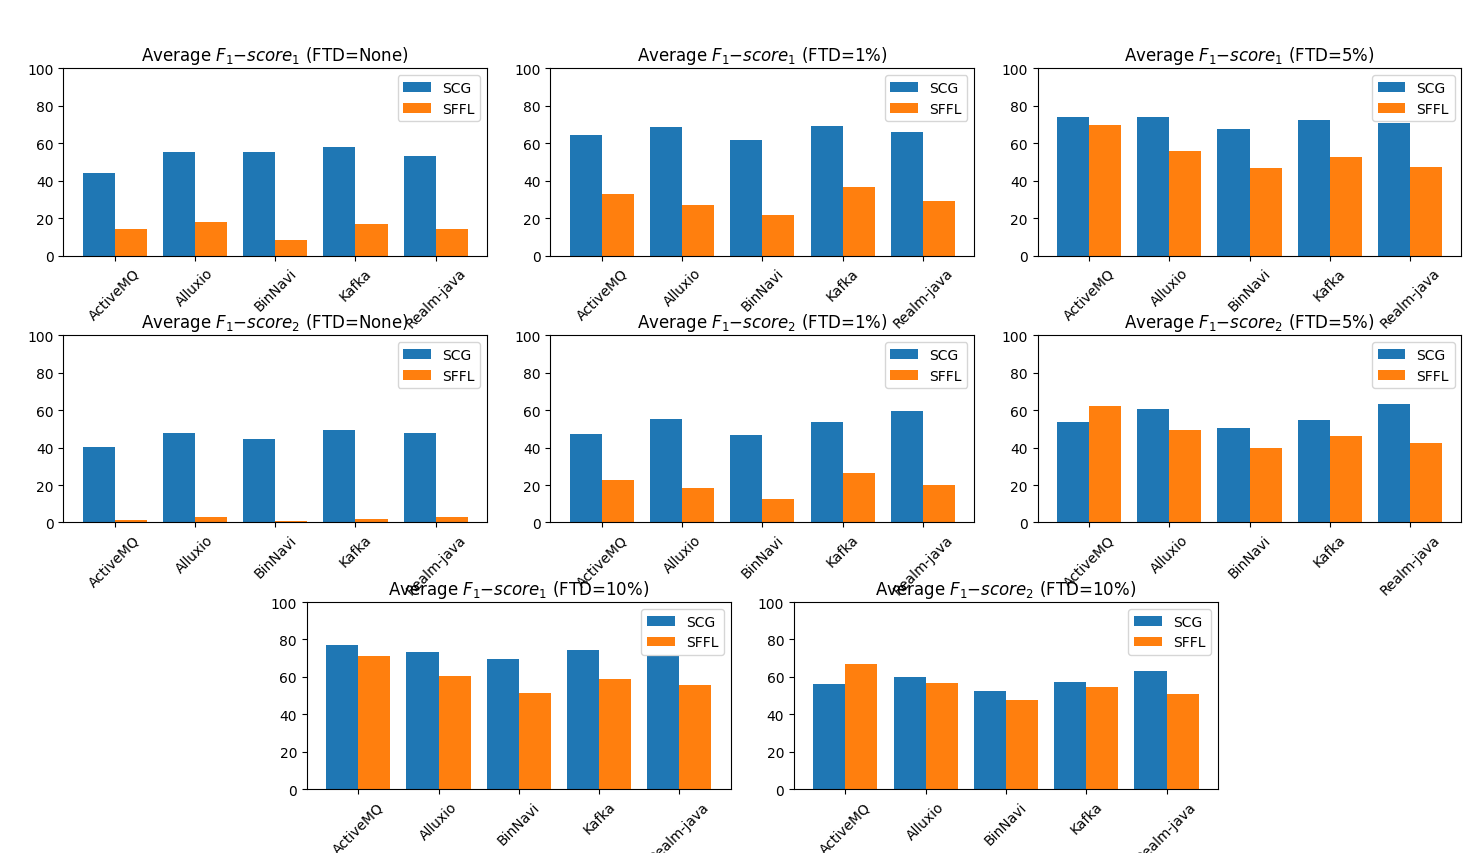
\includegraphics[width=1.0\textwidth]{SCGvsSFFL_F1_scores.png}
\caption{Performance comparison between SCG and SFFL across different fine-tuning scenarios using average $F_1$-scores}
\label{fig:scg_vs_sffl}
\end{figure}

\section{Threats to Validity}
We meticulously considered potential threats across several categories to ensure robust and valid results, addressing conclusion validity through careful statistical analyses, internal validity through rigorous model and feature selection, construct validity via representative datasets, and external validity through diverse testing environments.

\section{Related Work}
Traditional heuristic methods such as JDeodorant and JMove have limitations in scalability and accuracy. Our GNN-based methods represent a significant advancement, providing superior accuracy, deeper semantic analysis, and practical automated refactoring strategies.

\section{Conclusion}
We have introduced and validated a comprehensive GNN-based solution for detecting and refactoring feature envy. Our approach, utilizing SCG and SFFL, consistently outperformed traditional methods, achieving notable improvements in accuracy, generalization, and maintainability. Future directions include further optimization for larger projects and more detailed analysis of refactoring outcomes.

\end{document}
